\documentclass[border=12pt]{standalone}
\usepackage{tikz}
\usetikzlibrary{shapes.geometric, arrows.meta, positioning, calc, fit, backgrounds}
\usepackage{fontspec}
\usepackage{amsmath}
\setmainfont{DejaVu Sans}

\begin{document}
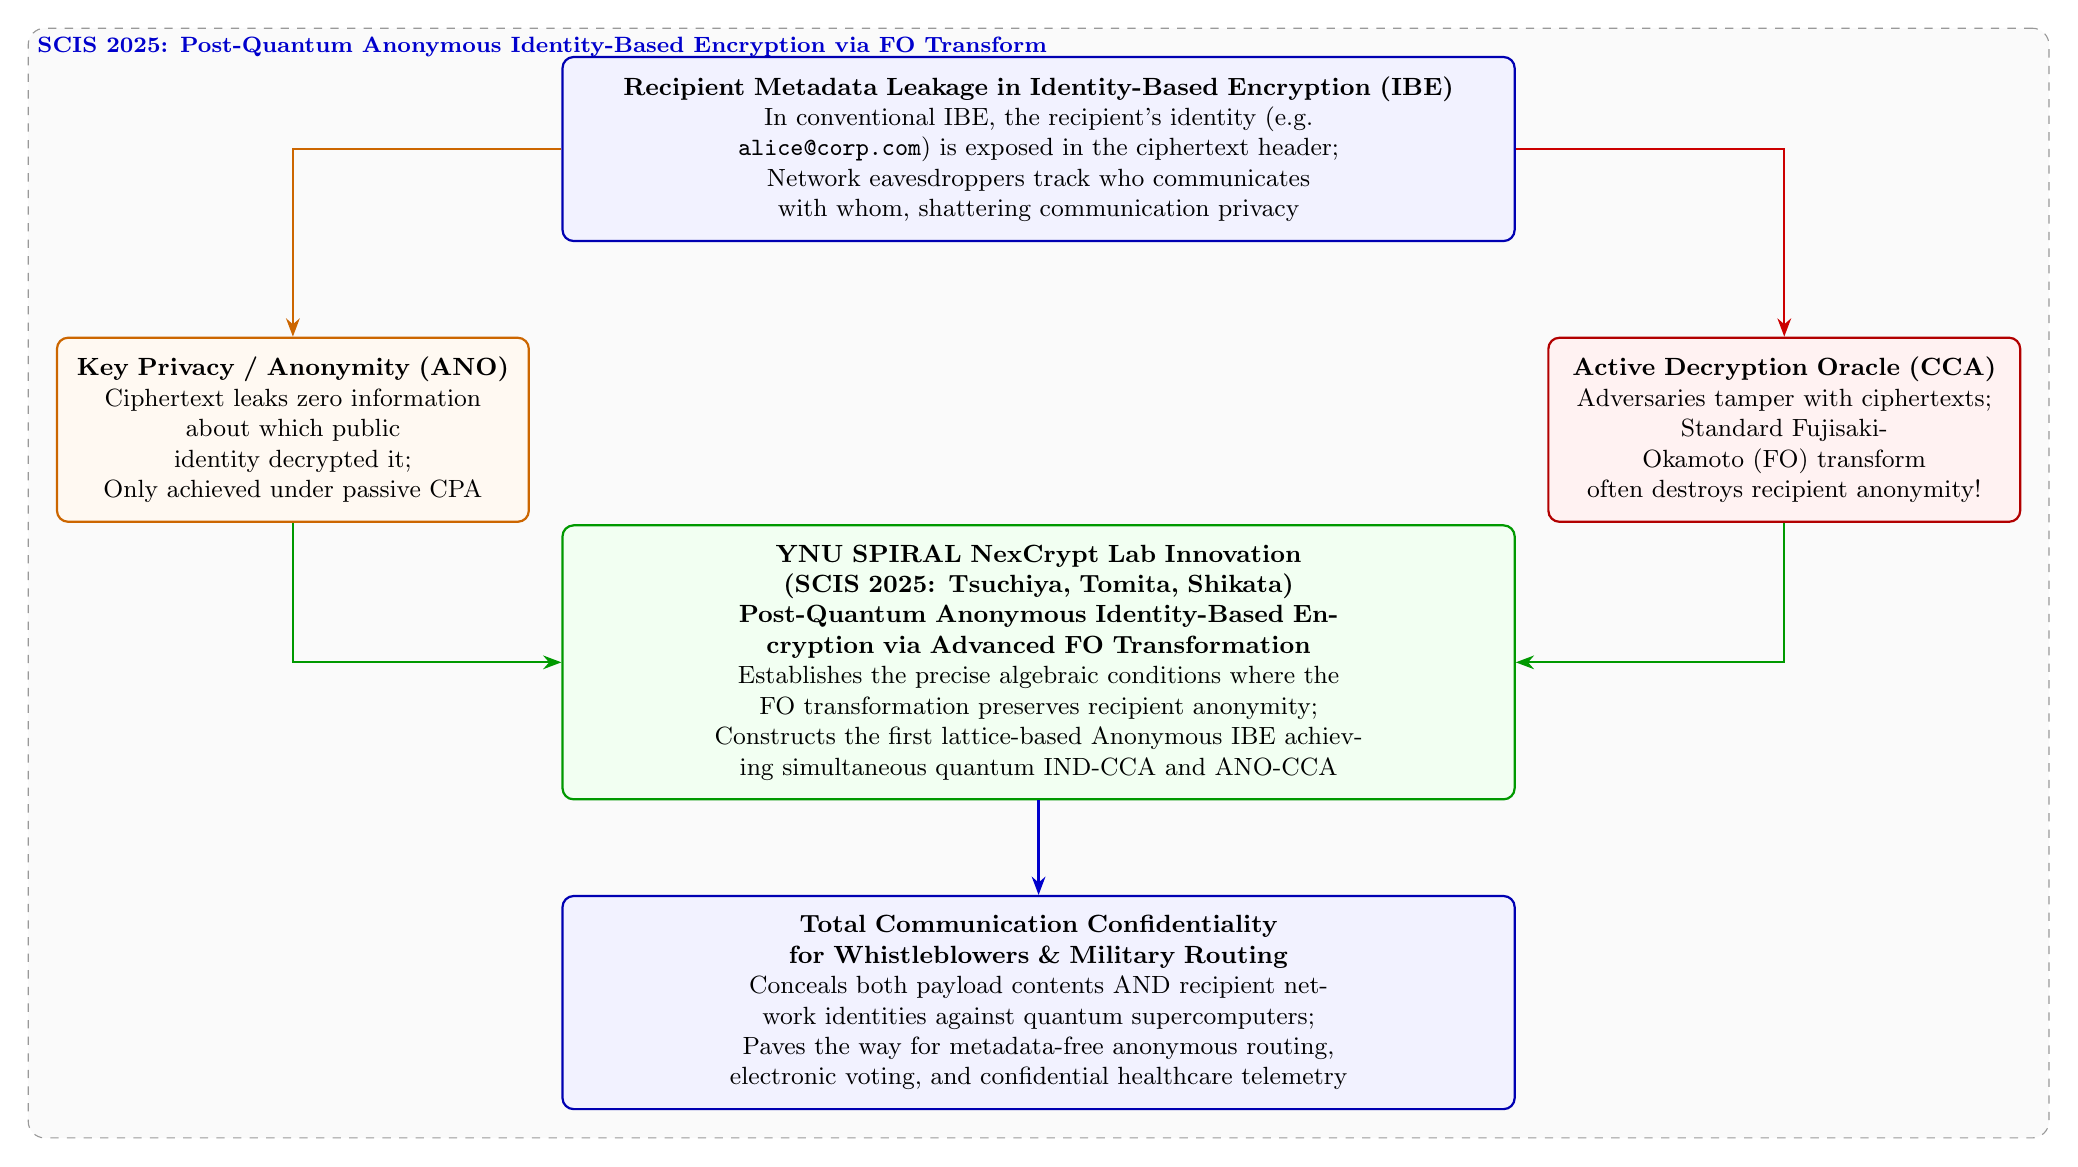
\begin{tikzpicture}[
    font=\small,
    >=Stealth,
    node distance=1.2cm,
    block/.style={rectangle, draw=blue!70!black, fill=blue!5, rounded corners=4pt, thick, align=center, inner sep=7pt},
    alertblock/.style={rectangle, draw=red!70!black, fill=red!5, rounded corners=4pt, thick, align=center, inner sep=7pt},
    greenblock/.style={rectangle, draw=green!60!black, fill=green!5, rounded corners=4pt, thick, align=center, inner sep=7pt},
    amberblock/.style={rectangle, draw=orange!80!black, fill=orange!5, rounded corners=4pt, thick, align=center, inner sep=7pt},
    groupbox/.style={draw=black!40, dashed, rounded corners=6pt, fill=black!2, inner sep=10pt}
]

    % Top: The Double Threat in ID-Based Cryptography
    \node[block, text width=11.6cm] (problem) {\textbf{Recipient Metadata Leakage in Identity-Based Encryption (IBE)}\\In conventional IBE, the recipient's identity (e.g. \texttt{alice@corp.com}) is exposed in the ciphertext header;\\Network eavesdroppers track who communicates with whom, shattering communication privacy};

    % Left: Classical CPA Anonymity
    \node[amberblock, below left=1.2cm and 0.4cm of problem, text width=5.5cm] (ano) {\textbf{Key Privacy / Anonymity (ANO)}\\Ciphertext leaks zero information\\about which public identity decrypted it;\\Only achieved under passive CPA};

    % Right: Active CCA Attacks
    \node[alertblock, below right=1.2cm and 0.4cm of problem, text width=5.5cm] (cca) {\textbf{Active Decryption Oracle (CCA)}\\Adversaries tamper with ciphertexts;\\Standard Fujisaki-Okamoto (FO) transform\\often destroys recipient anonymity!};

    \draw[->, thick, orange!80!black] (problem) -| (ano);
    \draw[->, thick, red!80!black] (problem) -| (cca);

    % Middle: YNU Breakthrough (SCIS 2025: Tsuchiya, Tomita, Shikata)
    \node[greenblock, below=1.2cm of $(ano)!0.5!(cca)$, text width=11.6cm] (breakthrough) {\textbf{YNU SPIRAL NexCrypt Lab Innovation (SCIS 2025: Tsuchiya, Tomita, Shikata)}\\\textbf{Post-Quantum Anonymous Identity-Based Encryption via Advanced FO Transformation}\\Establishes the precise algebraic conditions where the FO transformation preserves recipient anonymity;\\Constructs the first lattice-based Anonymous IBE achieving simultaneous quantum IND-CCA and ANO-CCA};

    \draw[->, thick, green!60!black] (ano) |- (breakthrough);
    \draw[->, thick, green!60!black] (cca) |- (breakthrough);

    % Bottom: Impact
    \node[block, below=1.2cm of breakthrough, text width=11.6cm] (impact) {\textbf{Total Communication Confidentiality for Whistleblowers \& Military Routing}\\Conceals both payload contents AND recipient network identities against quantum supercomputers;\\Paves the way for metadata-free anonymous routing, electronic voting, and confidential healthcare telemetry};

    \draw[->, thick, blue!80!black] (breakthrough) -- (impact);

    \begin{scope}[on background layer]
        \node[groupbox, fit=(problem) (ano) (cca) (breakthrough) (impact), label={[anchor=north west, font=\footnotesize\bfseries, blue!80!black]north west:SCIS 2025: Post-Quantum Anonymous Identity-Based Encryption via FO Transform}] {};
    \end{scope}

\end{tikzpicture}
\end{document}
